\section{Аналитический раздел} \label{analysis}

В данном разделе будут выдвинуты требования к приложению, определены пользователи системы, формализованы хранимые о системе данные, проведен анализ существующих моделей баз данных и осуществлен ее выбор.

\subsection{Требования к приложению}

Чтобы спортсмены имели возможность сразу же после выхода из воды взвесить улов, взвешивание и судейство происходит прямо на берегу водоемов, где возможность найти место и поставить ноутбук предоставляется редко. Разрабатываемое приложение было бы удобно использовать на более компактных устройствах, таких как телефон или планшет. В связи с чем выбор пал на платформу iOS --- создаваемое программное обеспечение будет разработано для смартфонов и электронных планшетов компании Apple.

Приложение должно поддерживать определенный функционал:
\begin{itemize}[label=---]
	\item персонализация для судей и администраторов;
	\item возможность входа без авторизации для спортсменов;
	\item формирование соревнований и их этапов;
	\item создание команды, деление участников по командам;
	\item добавление информации об улове участников;
	\item подсчет очков участников, команд;
	\item формирование личного и командного рейтингов;
	\item поиск определенного участника или конкретной команды.
\end{itemize}

\subsection{Пользователи системы}

В приложении будут представлены следующие роли:
\begin{enumerate}
	\item Участник --- пользователь, обладающий возможностью просматривать командный и личный рейтинги по любым этапам соревнований. Роль не требует авторизации.
	\item Судья --- пользователь, обладающий возможностями участника, а также возможностью создавать и удалять соревнования, создавать, редактировать и удалять участников, команды, добавлять участников в команды и удалять из команд, добавлять, редактировать и удалять уловы участников в этапы соревнований. Роль требует авторизации.
	\item Администратор ---  пользователь, обладающий возможностями участника и судьи, а также возможностью редактировать и удалять профили судей. Роль требует авторизации.
\end{enumerate}

На рисунке \ref{fig:UseCase} представлена диаграмма использования приложения.

\begin{figure}[h!]
	\centering{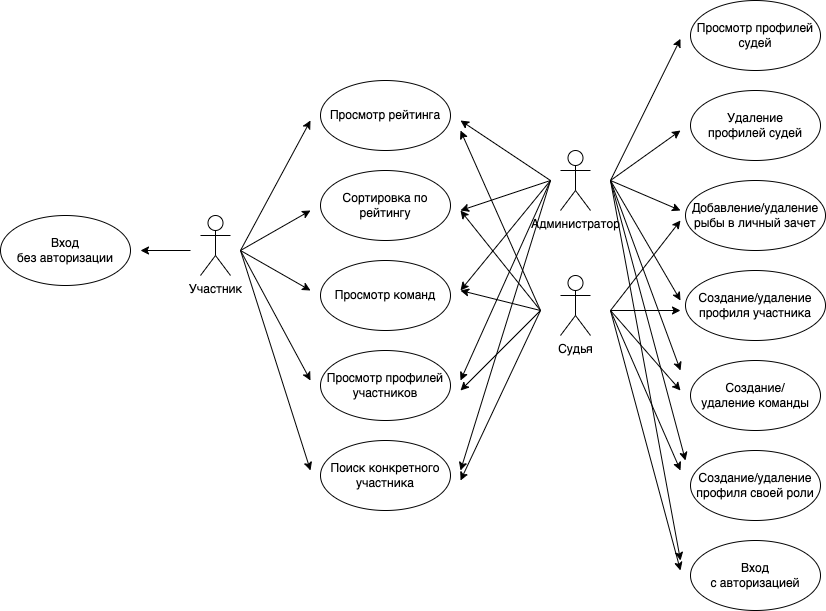
\includegraphics[scale=0.5]{img/UseCase.png}}
	\caption{Диаграмма использования приложения}
	\label{fig:UseCase}
\end{figure}

\subsection{Формализация данных}

База данных должна хранить информацию о следующих сущностях 

\begin{itemize}[label=---]
	\item соревнование;
	\item команда;
	\item участник;
	\item этап;
	\item название этапа;
	\item улов;
	\item рыба;
	\item роль;
	\item пользователь;
	\item авторизация.
\end{itemize}

В таблице \ref{decisions} представлены сущности и сведения о них.

\begin{table}[ht!]
	\centering
	\caption{Сущности и сведения о них}
	\label{decisions}
	\begin{tabular}{|p{4.3cm}|p{10.3cm}|}
		\hline
		\textbf{Сущность} & \textbf{Сведения}\\
		\hline 
		\ Участник & Фамилия, имя, отчество, команда, город, дата рождения, очки \\
		\hline 
		\ Команда & Название, соревнования, очки \\
		\hline 
		\ Соревнования & Название, команды \\
		\hline 
		\ Этап & Название этапа, участник, соревнование, очки \\
		\hline 
		\ Название этапа & Название \\
		\hline 
		\ Улов & Рыба, этап, вес, очки \\
		\hline 
		\ Рыба & Название \\
		\hline 
		\ Роль & Название \\
		\hline 
		\ Пользователь & Роль, авторизация  \\
		\hline 
		\ Авторизация & Логин, пароль \\
		\hline
	\end{tabular}
\end{table}

\subsection{Анализ моделей баз данных}

Модель данных --- это абстрактное, самодостаточное, логическое определение объектов, операторов и прочих элементов, в совокупности составляющих абстрактную машину доступа к данным, с которой взаимодействует пользователь. Эти объекты позволяют моделировать структуру данных, а операторы — поведение данных \cite{modeldb}. 

В настоящее время разработано множество моделей данных, рассмотрим основные из них.

\subsubsection{Иерархическая модель}

В иерархической модели данных используется представление базы данных в виде древовидной структуры, состоящей из объектов различных уровней. Между объектами существуют связи, каждый объект может включать в себя несколько объектов более низкого уровня. Такие объекты находятся в отношении предка к потомку, при этом возможна ситуация, когда объект--предок имеет несколько потомков, тогда как у объекта--потомка обязателен только один предок.

\subsubsection{Сетевая модель}

Сетевая модель базы данных подразумевает, что у родительского элемента может быть несколько потомков, а у дочернего элемента --- несколько предков. Структура такой модели представлена в виде графа, причем каждая вершина графа хранит экземпляры сущностей (записи одного типа) и сведения о групповых отношениях с сущностями других типов. Каждая запись может хранить произвольное количество значений атрибутов (элементов данных и агрегатов), характеризующих экземпляр сущности. Для каждого типа записи выделяется первичный ключ --- атрибут, значение которого позволяет однозначно идентифицировать запись среди экземпляров записей данного типа \cite{setmodel}.

\subsubsection{Реляционная модель}

Реляционная модель данных является совокупностью данных и состоит из набора двумерных таблиц. При табличной организации отсутствует иерархия элементов. Таблицы состоят из строк --- записей и столбцов --- полей. На пересечении строк и столбцов находятся конкретные значения. Для каждого поля определяется множество его значений. За счет возможности просмотра строк и столбцов в любом порядке достигается гибкость выбора подмножества элементов.

Наиболее популярными реляционными СУБД являются Oracle, Microsoft, SQL Server и PostgreSQL.

\subsection{Выбор СУБД}

Система управления базами данных, сокр. СУБД --- совокупность программных и лингвистических средств общего или специального назначения, обеспечивающих управление созданием и использованием баз данных \cite{subd}.

Основными функциями СУБД являются:

\begin{itemize}[label=---]
	\item управление данными во внешней памяти;
	\item управление данными в оперативной памяти с использованием дискового кэша;
	\item журнализация изменений, резервное копирование и восстановление базы данных после сбоев;
	\item поддержка языков БД.
\end{itemize}

Для ускорения быстродействия разрабатываемого приложения, можно прибегнуть к кэшированию данных. Для кэширования данных можно использовать NoSQL \cite{nosql} in--memory базы данных. Такие базы данных хранят данные в оперативной памяти, что обеспечивает более быстрый доступ к данным.

Основными решениями интеграции баз данных в мобильные приложения под iOS являются SQLite, Firestore и Realm.

\subsubsection{SQLite}

SQLite --- это встроенная в процесс библиотека, которая реализует автономный, бессерверный транзакционный компонент SQL  \cite{sqlite}. Код для SQLite находится в общественном достоянии и, таким образом, свободен для использования в любых целях. SQLite --- это встроенный движок базы данных SQL. 

В отличие от большинства других баз данных SQL, SQLite не имеет отдельного серверного процесса. Транзакции являются ACID, даже если они прерваны системными сбоями или сбоями питания. SQLite 

\subsubsection{Firestore}

Cloud Firestore --- это NoSQL, ориентированная на документы база данных. В отличие от базы данных SQL, здесь нет таблиц или строк. Вместо этого вы храните данные в документах, которые организованы в коллекции \cite{firebase}.

Каждый документ содержит набор пар ключ--значение. Облачное хранилище Firestore оптимизировано для хранения больших коллекций небольших документов.

Все документы должны храниться в коллекциях. Документы могут содержать вложенные коллекции и вложенные объекты, оба из которых могут включать примитивные поля, такие как строки, или сложные объекты, такие как списки.

Коллекции и документы создаются неявно в Cloud Firestore. Просто назначьте данные документу в коллекции. Если коллекция или документ не существуют, Cloud Firestore создает их.

\subsubsection{Realm от MongoDB}

Realm --- это реактивная, объектно-ориентированная, кроссплатформенная, NoSQL мобильная база данных \cite{realm}. 

Файлы Realm содержат объектные данные со следующими структурами данных: группы, таблицы, деревья кластеров и кластеры. База данных Realm организует эти структуры данных в древовидную структуру следующего вида:

\begin{itemize}[label=---]
	\item верхний уровень, известный как Группа, хранит метаданные объекта, журнал транзакций и коллекцию таблиц;
	\item каждый класс в схеме realm соответствует таблице в группе верхнего уровня;
	\item каждый таблица содержит дерево кластеров, реализацию дерева B +;
	\item листья на дереве кластеров называются кластерами, каждая содержит диапазон объектов, отсортированных по значению ключа;
	\item кластеры хранят объекты в виде наборов столбцов.
\end{itemize}

База данных Realm гарантирует, что транзакции совместимы с ACID, а также имеет удобный SDK для внедрения в мобильные приложения.

\subsubsection{Выбор СУБД}

NoSQL базы данных набирают популярность, причиной чему является простота разработки, функционала и высокая производительности. В связи с наличием интереса к данному подходу проектирования систем, а также из--за наличия удобного SDK для iOS, был выбран Realm от MongoDB.

\subsection{Вывод из раздела}

В данном разделе были выделены ролевые модели системы, конкретизированы данные и их связь между собой, построены соответствующие диаграммы. Был проведен анализ и выбор модели данных, а также СУБД, подходящей для решения поставленной задачи. 
